\documentclass[
	handout,
	hyperref={unicode, colorlinks=true, linkcolor=.}
]{beamer}
% \usetheme{rochester}


%%% ENCODING, FONT & LOCALIZATION
\usepackage[utf8]{inputenc} % use unicode input-encoding (allows unicode characters in the .tex files, default: Asci)
\usepackage{lmodern} % vectorized version of the "computer modern" font (default) (https://tex.stackexchange.com/q/1390/148164, https://tex.stackexchange.com/q/147194/148164)
\usepackage[ngerman, english]{babel} %% last language is main
%\shorthandoff{"} %babel breaks tikz-cd otherwise (activate if used)
\usepackage{csquotes} %% biblatex wants csquotes (localized quotes) if babel is present

%%% GENERAL IMPROVEMENTS
\usepackage[unicode, colorlinks=true, linkcolor=.]{hyperref} %% clickable links
\usepackage{enumitem} %% better (customizable) enumerations (e.g. \begin{enumerate}[label=(\roman*)])


%%% STYLING
% \setlength{\parindent}{0em} % No indentation for new paragraphs
\usepackage{emptypage} % removes page numbers on empty pages
% \makeatletter \@twosidefalse \makeatother
\usepackage{xcolor}


%%% GRAPHICS & PLOTS

% \usepackage{graphicx} % enable pictures
\usepackage{wrapfig} % text wrapping around figures
% \usepackage{tikz, tikz-cd, pgfplots} % plots and sketches
% \pgfplotsset{compat=1.16}

%%% CODE
\usepackage[ruled,linesnumbered]{algorithm2e}

% fix algomathdisplay (see: https://tex.stackexchange.com/a/611426/148164)
\makeatletter
\renewenvironment{algomathdisplay}
 {\[}
 {\@endalgocfline\vspace{-\baselineskip}\]{\DontPrintSemicolon\;}}
\makeatother
%%% MATH
\usepackage{mathtools} % fixes some things from amsmath and adds some new features
\usepackage{amsthm, amssymb} % amsthm -> proof env, amssymb -> additional symbols
\usepackage{aligned-overset} % https://tex.stackexchange.com/questions/257529/overset-and-align-environment-how-to-get-correct-alignment
%% usage: \overset{something}&{=}

%%% Special Symbols
% \usepackage{bbm} % blackboard numbers: usage \mathbbm{1} (amssymb \mathbb{1} looks bad)
\usepackage{cancel} % strike through equation parts to indicate they cancel out
% %% contradiction symbol
% \usepackage{wasysym} % lightning symbol
% \newcommand*{\contradiction}[1][]{\quad\text{{\LARGE\lightning} #1}\ }

%%% EDITING (Annotations, TODO, etc.) 
\usepackage[draft]{fixme} %final removes annotations %draft includes annotations
\fxsetup{theme=color}
%%\fxnote{some note} ,\fxwarning{}, \fxerror{}, \fxfatal{} <- does not allow [final] to compile

%%% BIBLIOGRAPHY
\usepackage[style=alphabetic, backend=biber, seconds=true, date=iso, urldate=iso, maxcitenames=2]{biblatex}
\addbibresource{references.bib}

%% AMS Theorem Environments

%% REPEATABLE THEOREMS
%% cf. https://tex.stackexchange.com/a/443/148164
\makeatletter
\newcommand{\newreptheorem}[2]{% define repeatable theorems
	\newtheorem*{rep@#1}{\rep@title} %  -> no number, special title

	\newenvironment{rep#1}[1]{% define repetition environement with required label-reference
		\def\rep@title{#2 \ref{##1}} % use reference to define title
		\begin{rep@#1} % begin second occasion with correct title definition
	}{
		\end{rep@#1}
	}
}
\makeatother

\newreptheorem{test}{Test}
\theoremstyle{plain}% default
\newtheorem{prop}{Proposition}[section]
\newtheorem{lemma}[prop]{Lemma}
\newreptheorem{lemma}{Lemma}
\newtheorem{corollary}[prop]{Corollary}
\newtheorem{theorem}[prop]{Theorem}

\theoremstyle{definition}
\newtheorem{definition}[prop]{Definition}
\newtheorem{example}[prop]{Example}
\newtheorem{assumption}[prop]{Assumption}
\newtheorem{axiom}[prop]{Axiom}

\theoremstyle{remark}
\newtheorem{remark}[prop]{Remark}



%%
\newcommand*{\real}{\mathbb{R}}
\newcommand*{\dimension}{d}

\newcommand*{\Rom}[1]{\text{\RN{#1}}} % uppercase roman numbers
\newcommand*{\rom}[1]{\text{\Rn{#1}}} % lowercase roman numbers

\newcommand*{\E}{\mathbb{E}}
\renewcommand{\Pr}{\mathbb{P}}
\DeclareMathOperator{\sgn}{sgn}
\newcommand*{\identity}{\mathbb{I}}
\newcommand*{\Loss}{\mathcal{L}}
\newcommand*{\loss}{\ell}
\newcommand*{\param}{\theta}
\newcommand{\model}[2][\param]{f(#1, #2)}
\DeclareMathOperator*{\argmin}{argmin}
\DeclareMathOperator*{\argmax}{argmax}

\newcommand*{\step}{\mathbf{d}}
\newcommand*{\lr}{\eta}
\newcommand*{\ubound}{L}
\DeclareMathOperator{\LUE}{\hyperref[def: LUE]{LUE}} % Set of Linear Unbiased Estimators
\DeclareMathOperator{\BLUE}{\hyperref[def: BLUE]{BLUE}} % Best Linear Unbiased Estimator
\DeclareMathOperator{\EI}{EI} % Expected Improvement
\DeclareMathOperator{\KG}{KG} % Knowledge Gradient
\newcommand*{\variogram}{\hyperref[def: variogram]{\gamma}}


\DeclareMathOperator{\linHull}{Lin}
\DeclareMathOperator{\Cov}{Cov}
\DeclareMathOperator{\Var}{Var}
\newcommand*{\C}{\hyperref[def: covariance function]{\mathcal{C}}} % Covariance function
\newcommand*{\sqC}{C} % isotropic Covariance function


\newtheorem*{remark}{Remark}


\title{Using Statistics to Determine the Learning Rate for Gradient Descent}
\author{Felix Benning}
\institute{University of Mannheim}

\begin{document}
	\frame{\titlepage}

	\begin{frame}{Outline}
		\tableofcontents
	\end{frame}

	\AtBeginSection[]
	{
	\begin{frame}{Outline}
		\tableofcontents[currentsection]
	\end{frame}
	}

	\section{Motivation}

		\begin{frame}{Optimization by Approximation}

	Goal: Optimize Loss \(\Loss\)

	\begin{algorithm*}[H]
		\caption{Optimization by Approximation}
		\KwIn{starting point \(\param\)}
		\While{not converged}{
			\(\hat{\Loss} \leftarrow\) Approximation of \(\Loss\) around \(\param\)

			\(\param \leftarrow \argmin_{\param} \hat{\Loss}(\param)\)
		}
	\end{algorithm*}
\end{frame}
		
\begin{frame}{Newton-Raphson}
	Second order Taylor
	\begin{align*}
		\hat{\Loss}_{N}(\param + \step)
		&:= T^2_\param \Loss(\param + \step)\\
		&= \Loss(\param)
		+ \langle \grad\Loss(\param), \step\rangle
		+ \tfrac12 \langle \grad^2\Loss(\param) \step, \step\rangle
	\end{align*}
\only<2->{
	leads to \textbf{Newton-Raphson}
	\begin{equation*}
		\step^*_{N} := -[\grad^2\Loss(\param)]^{-1}\grad\Loss(\param)
		= \argmin_\step \hat{\Loss}_{N}(\param + \step).
	\end{equation*}
}
\end{frame}

		\begin{frame}{Gradient Descent}
	Assuming \(\hessian\Loss \preceq \ubound\identity\) implies
	\only<1-2>{
		\begin{align*}
			|\Loss(\param+\step) - T^1_\param \Loss(\param+\step)|
			&= \left| \frac 12 \int_0^1 \step^T \grad^2\Loss(\param + \lambda \step)\step d\lambda\right|\\
			&\le \tfrac{\ubound}2 \|\step\|^2.
		\end{align*}
	}
	\only<2>{Therefore we have}
	\only<2->{
		\begin{equation*}
			\Loss(\param + \step) \le \hat{\Loss}_G(\param+\step)
			:= T^1_\param \Loss(\param+\step) + \tfrac{\ubound}2\|\step\|^2.
		\end{equation*}
	}
	\only<3>{
		This results in \textbf{gradient descent}
		\begin{equation*}
			\step^*_{G} := - \frac1\ubound \grad\Loss(\param)
			= \argmin_\step \hat{\Loss}_{G}(\param + \step).
		\end{equation*}
	}
\end{frame}

		\begin{frame}{Determining the Learning Rate}
	\setbeamersize{description width=0.57cm}

	\begin{enumerate}
		\item Estimation
		\begin{description}
		\only<1-6>{
			\only<1->{
				\item[Q:] For how long can we trust \(\grad\Loss(\param)\),
				i.e. the first taylor approximation?
			}
			\only<2->{\item[A:] Depends on how fast the gradient changes}
			\only<3->{\item[Q:] How fast does the gradient change?}
			\only<4->{\item[A:]
				\(\hessian\Loss \preceq \ubound\identity\) represents a trust bound because
				\[
					\grad\Loss(\param+\step) - \grad\Loss(\param)
					= \int_0^1 \hessian\Loss(\param + \lambda \step)\step d\lambda
				\]
			}
			\only<5->{\item[Q:] Can we just use \(\hessian\Loss(\param)\) to estimate that integral?}

		}
			\only<6->{\item[A:] Recursion}
		\end{description}

		\only<7-|handout:0>{
			\item Religious Belief:

			``I believe that \(\hessian\Loss(\param)\preceq
			\ubound\identity\)'' therefore I set the learning rate
			\[
				\lr=\tfrac1\ubound
			\]
		}
		\only<8->{
			\item Trial \& Error
			\begin{description}
				\item[fast:] Backtracking \parencite{truongBacktrackingGradientDescent2019}
			\only<9->{
				\item[slow:] ``Hyperparemeter Tuning'' (\(\rightarrow\) Bayesian
				Optimization \parencite{frazierBayesianOptimization2018})
			}
			\end{description}
		}
	\end{enumerate}
\end{frame}
		\begin{frame}{Where This is Going}
	\begin{center}
		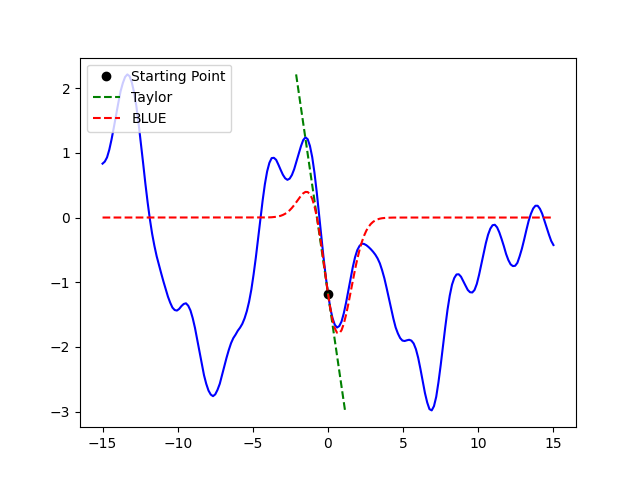
\includegraphics[scale=0.65]{graphics/BLUEvsTaylor3.png}
	\end{center}
\end{frame}

	\section{Preliminaries}

		\subsection{Random Fields}
		\begin{frame}{Random Fields}
	\begin{definition}[Random Field]
		A family of random variables \((Z(x))_{x\in\real^\dimension}\) is a
		\emph{random field} over \(\real^\dimension\).
	\end{definition}
	\begin{definition}[Covariance Function]\label{def: covariance function}
		The covariance function \(\C\) of a random field \(Z\) is defined as
		\[
			\C(x,y) = \Cov(Z(x),Z(y))	
		\]
		\vspace*{-0.5cm}	
		\begin{enumerate}
			\item \(Z\) is \emph{stationary} if \(\C(x,y) = \C(x-y)\).
			\item \(Z\) is \emph{intrinsically stationary} if its increments
			\(Z_\step(x) = Z(x+\step) - Z(x)\) are stationary. Then the
			\emph{variogram} is defined as
			\begin{equation*}\label{def: variogram}
				\variogram(\step) := \tfrac12\Var(Z_\step(x)) = \tfrac12\Var(Z_\step(0))
			\end{equation*}
		\end{enumerate}
	\end{definition}
\end{frame}
		\begin{frame}{Random Field Derivative}
	\begin{definition}
		If there exists a (square integrable) random field \(Z'\), such that for
		all \(x\) we have
		\[
			\E\left[\bigg(\frac{Z(x+h)-Z(x)}{h}-Z'(x)\bigg)^2\right] \to 0 \quad (h\to 0),
		\]	
		then \(Z'\) is the derivative of the (square integrable) random field
		\(Z\).
	\end{definition}

\only<2->{
	\begin{theorem}[{\cite[Section 5.3.2]{scheurerComparisonModelsMethods2009}}]
		\begin{center}
		\(Z\) is differentiable \(\iff\) \(\partial_x\partial_y\C(x,y)\) exists	
		\end{center}
		We have
		\begin{align*}
			\Cov(Z'(x), Z'(y)) &= \partial_x\partial_y \C(x,y)
\only<3->{
			&&= -\C''(x-y)
}			\\
			\Cov(Z'(x), Z(y)) &= \partial_x\C(x,y)
\only<3->{
			&&= \C'(x-y)
}
		\end{align*}
	\end{theorem}
}
	 
\end{frame}

		\subsection{BLUE}
		\begin{frame}{BLUE}
\only<1-2>{
	A \textbf{linear estimator}
	\(\hat{Y}\) of \(Y\) using \(X_1,\dots,X_n\) is of the form 
	\begin{equation*}
		\hat{Y}\in \linHull\{X_1,\dots,X_n\} + \real.
	\end{equation*}
}\only<2-3>{
	The set of \textbf{unbiased linear estimators} is defined as
	\begin{align*}\label{def: LUE}
		\LUE
		&= \{ \hat{Y} \in \linHull\{X_1,\dots,X_n\} + \real : \E[\hat{Y}] = \E[Y]\}\\
		\nonumber
		&= \{ \hat{Y} - \E[\hat{Y}] + \E[Y] : \hat{Y} \in \linHull\{X_1,\dots,X_n\}\}.
	\end{align*}
}\only<3->{
	And the BLUE is the \textbf{best linear unbiased estimator}, i.e.
	\begin{equation*}\label{def: BLUE}
		\BLUE[Y\mid X_1,\dots, X_n] := \argmin_{\hat{Y}\in\LUE} \E[\|\hat{Y} - Y\|^2].
	\end{equation*}
}\only<4->{
	
\begin{lemma}\label{lem: blue is cond. expectation}
	If \(X,Y_1,\dots, Y_n\) are multivariate normal distributed, then we
	have
	\begin{align*}
		\BLUE[Y\mid X_1,\dots,X_n]
		&= \E[Y\mid X_1,\dots, X_n]\\
		\bigg(&=
		\argmin_{\hat{Y}\in\{f(X_1,\dots, X_n) : f\text{ meas.}\}} \E[\|Y-\hat{Y}\|^2]
		\bigg).
	\end{align*}
\end{lemma}
	
}
\end{frame}

	\section{Main Results}

		\begin{frame}{BLUE of the Loss (Stationary)}
	\scalebox{0.89}{
		\begin{minipage}{1.1\textwidth}
			
\begin{lemma}\label{lem: blue centered, stationary}
	If \(\Loss\) is a \textbf{stationary, centered, differentiable} random field
	with covariance function \(\C\), then
	\begin{align*}
		\BLUE[\Loss(\param + \step)\mid \Loss(\param), \grad\Loss(\param)]
		&= \frac{\C(\step)}{\C(0)} \Loss(\param)
		+ \grad\C(\step)^T [\grad^2\C(0)]^{-1} \grad\Loss(\param)
	\\
	\intertext{
		if additionally \(\Loss\) is \textbf{isotropic}, i.e.
		\(\C(\step)=\sqC(\|\step\|^2)\), this reduces to
	}
		&= \frac{\sqC(\|\step\|^2)}{\sqC(0)} \Loss(\param)
		+ \frac{\sqC'(\|\step\|^2)}{\sqC'(0)} \langle \step, \grad\Loss(\param)\rangle.
	\end{align*}
\end{lemma}

		\end{minipage}
	}
\end{frame}
		\begin{frame}{BLUE of the Loss (Intrinsically Stationary)}
	
\begin{lemma}\label{lem: blue centered, intrinsically stationary}
	If \(\Loss\) is a \textbf{centered, intrinsically stationary, differentiable}
	random field, with variogram \(\variogram\), then
	\begin{align*}
		\BLUE[\underbrace{\Loss(\param+\step) - \Loss(\param)}_{=:\Loss_\param(\step)}
		\mid \grad\Loss(\param)]
		&=  \grad\variogram(\step)^T[\grad^2\variogram(0)]^{-1}
		\grad\Loss(\param)\\
		\intertext{
			if the variogram is \textbf{rotation invariant}, i.e.
			\(\variogram(\step)=\phi(\|\step^2\|)\), this simplifies to
		}
		&= \frac{\phi'(\|\step\|^2)}{\phi'(0)}
		\langle \step, \grad\Loss(\param)\rangle
	\end{align*}
\end{lemma}

\end{frame}


		\begin{frame}{Bayesian Descent}
	\begin{theorem}[Bayesian Descent]\label{thm: bayesian descent}
		Gradient descent, i.e. 
		\begin{equation*}
			\step(\lr) = - \tilde{\lr} \grad\Loss(\param)
			= - \frac{\lr}{\|\grad\Loss(\param)\|} \grad\Loss(\param)
		\end{equation*}
		minimizes the 1-step 0-order \(\BLUE\) of rotation invariant random fields
		\(\Loss\) in the following sense
		\begin{itemize}
		\alt<2>{
			\item for a \textbf{centered, intrinsically stationary, differentiable}
			random field \(\Loss\) with \textbf{rotation invariant} variogram
			\(\variogram(\step) = \phi(\|\step\|^2)\), we have
			\begin{align*}
				\step(\hat{\lr})
				&= \argmin_{d}
				\BLUE[\Loss(\param + \step) - \Loss(\param)\mid \grad\Loss(\param)]\\
				\hat{\lr}
				&= \argmax_{\lr} \lr\frac{\phi'(\lr^2)}{\phi'(0)}
			\end{align*}
		}{
			\item for a \textbf{centered, isotropic} random field \(\Loss\) with
			\(\C(\step)=C(\|\step\|^2)\), we have
			\begin{align*}
				\step(\hat{\lr})
				&= \argmin_{d}
				\BLUE[\Loss(\param + \step)\mid \Loss(\param), \grad\Loss(\param)]\\
				\hat{\lr}
				&= \argmin_{\lr}\frac{\sqC(\lr^2)}{\sqC(0)} \frac{\Loss(\param)}{\|\grad\Loss(\param)\|}
				-  \lr\frac{\sqC'(\lr^2)}{\sqC'(0)}
			\end{align*}
		}
		\end{itemize}
	\end{theorem}
\end{frame}

	\section{Covariance Models}
		\begin{frame}{Squared Exponential}
	
\begin{theorem}
	For a \textbf{centered} random field \(\Loss\) with \textbf{squared exponential}
	covariance function
	\[
		\C(\step) = \sigma^2 e^{-\frac{\|\step\|^2}{2\scale^2}},
	\]
	we have
	\begin{equation*}
		\step(\hat{\lr})
		= \argmin_{\step} \BLUE[\Loss(\param + \step)\mid \Loss(\param),\grad\Loss(\param)]
	\end{equation*}	
	with
	\begin{equation*}
		\hat{\lr}
		= \frac{\Loss(\param)}{2\|\grad\Loss(\param)\|}
		+ \sqrt{
			\left(\frac{\Loss(\param)}{2\|\grad\Loss(\param)\|}\right)^2 + \scale^2 
		}.
	\end{equation*}
\end{theorem}

\end{frame}
		\begin{frame}{The Matérn Covariance Model}

\end{frame}
		\begin{frame}{Matérn}
	
\begin{theorem}
	Assuming \(\Loss\) is a \textbf{centered} random field with \textbf{Matérn}
	covariance \(\C_{p+\frac12}\) for \(p\in\nat\), we have for
	\(\Loss(\param)\le 0\)
	\begin{equation*}
		\step(\hat{\lr})
		= \argmin_{d}
		\BLUE[\Loss(\param + \step) \mid \Loss(\param), \grad\Loss(\param)]
	\end{equation*}
	with
	\begin{itemize}
		\item \(p=1\)
		\begin{equation*}
			\hat{\lr}
			= \frac{s}{\sqrt{3}}\frac{1}{\left(
				1- \frac{\sqrt{3}}{s}\frac{\Loss(\param)}{\|\grad\Loss(\param)\|}
			\right)}
		\end{equation*}

		\item \(p=2\)
		\begin{equation*}
			\hat{\lr}
			= \frac{s}{2\sqrt5} \left(
				1 + \sqrt{1+\frac4{1-\frac{\sqrt{5}}{3s}\frac{\Loss(\param)}{\|\grad\Loss(\param)\|}}}
			\right)
		\end{equation*}
	\end{itemize}
\end{theorem}
	
\end{frame}

		\begin{frame}{The Schlather-Moreva Model}
	\begin{equation*}
		\variogram_{\alpha,\beta}(\step)
		= \frac{(1+\|\step\|^\alpha)^{\beta/\alpha}-1}{2^{\beta/\alpha}-1}
		\quad \alpha\in (0,2],\ \beta\in(-\infty, 2].
	\end{equation*}
	\begin{itemize}
		\item Fractional Brownian Motion \(\variogram_{\alpha,\alpha}(\step)=\|\step\|^\alpha\) for \(\alpha=\beta\).
		\item Differentiable for \(\alpha=2\).
		\item Can be stationary for \(\beta<0\). 

		I.e. we can define
		\[
			\C_\beta(\step) := c_\beta - \variogram_{2,\beta}(\step)
		\]
		with \(c_\beta := \lim_{\|\step\|\to\infty}\variogram_{2,\beta}(\step)\).
		A random field with this covariance function will have variogram
		\(\variogram_{2,\beta}\).
	\end{itemize}
\end{frame}
		\begin{frame}[allowframebreaks]{Schlather-Moreva}
	
\begin{theorem}[Intrinsically Stationary]
	Assuming \(\Loss\) is centered and has variogram \(\variogram_{2,\beta}\)
	with \(\beta\in(-\infty, 1]\), we have
	\begin{align*}
		\step(\hat{\lr})
		&= \argmin_{d}
		\BLUE[\Loss(\param + \step) - \Loss(\param)\mid \grad\Loss(\param)]\\
		\hat{\lr}
		&= \frac1{\sqrt{1-\beta}}.
	\end{align*}
\end{theorem}


	\framebreak

	
\begin{theorem}[Stationary]
	Assuming \(\Loss\) is centered, has covariance \(\C_\beta\) with
	\(\beta\in(-\infty, 0)\), then we have for \(\Loss(\param)\le 0\)
	\begin{align*}
		\step(\hat{\lr})
		&= \argmin_{d}
		\BLUE[\Loss(\param + \step) \mid \Loss(\param), \grad\Loss(\param)]\\
		\hat{\lr}
		&= \Root_\lr\left(
			-1 + \frac{\beta\Loss(\param)}{\|\grad\Loss(\param)\|}\lr
			+(1-\beta)\lr^2 + \frac{\beta\Loss(\param)}{\|\grad\Loss(\param)\|}\lr^3
		\right).
	\end{align*}
	The unique root can be found either by solving the polynomial of third degree
	(e.g. using Cardano's method) or by bisection as the root is in \([0,
	1/\sqrt{1-\beta}]\) and the function is monotonously increasing.
\end{theorem}

\end{frame}

	\appendix

	\begin{frame}[allowframebreaks]{Bibliography}
		\printbibliography
	\end{frame}
\end{document}